\cotefile{154}
\scanpage{46}
% E: text|upper left, continuation|immersion des D_i
\unsure{immersion} des \(D_i\) dans \(\widetilde X\). (\unsure{à ne pas confondre avec le revêtement des bords de \(D_i\), qui est induit par choix d'orientation de \(D_i\)})

% E: text|left, i|On a une application
\textcircled{i} On a une application
% E: diagram|left below i|X phi Y
\diagram{\begin{tikzcd}X\arrow[r,"\varphi"]&Y.\end{tikzcd}}
(application \unsure{structurale})\inserted{\unsure{appellons|appellée} \deleted{\unsure{contraction}}} telle que

% E: text|left, numbered condition 2|La restriction
\unsure{2}) La restriction de \(\varphi\) à \unsure{\(\forall\) face} de \((X,K)\) est un \deleted{\unsure{polygone}}\inserted{isom.}

% E: text|left, cancelled condition 1|L'image de
\deleted{1) L'image \unsure{de \(\varphi\) est un \(\unsure{Y}\) qui est} \(X\setminus K\)}

% E: text|left, middle|Au voisinage
Au voisinage de l'un \deleted{\unsure{\(\forall\) point de \(K\setminus S(K)\)}}\inserted{\unsure{des arêtes de \(K\)}}, \(\varphi\) a la structure d'un ``folding'' d'arête.
\margin{\deleted{\unsure{Les seuls points qui contiennent deux composantes}} \unsure{Les faces exceptionnelles pour lesquelles}\inserted{\unsure{contour}} \unsure{contient un point de \(S\)}.}

% E: text|left, numbered condition 3|Au voisinage des
3) Au voisinage des \unsure{\(\forall\)} \deleted{\(\unsure{s}\)} sommets de \(K\), \(\varphi\) \unsure{a} la structure d'un \deleted{\(\unsure{\varphi}\)} ``double folding'' actif : \(s\) et les deux branches de \(K\) passant en \(s\).

% E: text|left, numbered condition 4|L'image des
4) \deleted{L'image des \unsure{\(\forall\) sommets est} \(\varphi^{-1}(\bigcup D_i)\cap K=\unsure{S(L)}\cap\)}
% E: display|left lower, definition L|L = phi inverse union D_i
\[
L=\varphi^{-1}(\underbrace{\bigcup D_i}_{X_1\,\deleted{\unsure{\varphi}}})
\]
\margin{\unsure{Considérer qu'il faut se placer en dehors des ``voisins'' autour des composantes de \(K_0\)}.}
\deleted{\(\Longrightarrow\varphi^{-1}(\unsure{X_1})\cap K\)}

% E: text|lower left, corollary|Cor.
Cor. \inserted{\unsure{Pour}} \unsure{les pts de} \(S(K)\cap L=(\varphi|K)^{-1}(X_1)\), \deleted{\unsure{\(\forall\)}} \(\varphi(s)\) est un sommet, ssi \deleted{\(s\) est un sommet de} \inserted{\(s\) est \unsure{lui-$=$} un} \unsure{sommet de \(K\), et est un sommet de \(L\)} \deleted{\(L\) \unsure{lequel est le sommet critique de}} --- i.e. est un \uline{point critique} de \(K\) (l'un des \unsure{pts est en corr. 1--1 avec l'un des côtés ordinaires de \(K\)}).

% E: text|right top, j|Soit F une face
\deleted{\unsure{Soit}}
j) Soit \(F\) une face de \((X,K)\). Considérons les \deleted{\unsure{sommets}}\inserted{pts} critiques de \(K\) sur \(\delta F\), tels que le bord marqué en \uline{\(s\) (cf. (d))} \(\unsure{C_s}\) soit extérieur à \(F\), et corrigeons le contour \(\delta F\) par un petit renflement \deleted{\unsure{marqué}}\inserted{de façon} à ce que \(s\) soit du côté privilégié de \(s\).

% E: drawing|middle right, local contour correction|s
\figure{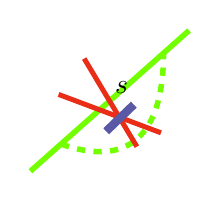
\begin{tikzpicture}[scale=.65]
\draw[green!55!yellow,line width=2pt](-1.6,-1.2)--(1.5,1.55);
\draw[green!55!yellow,line width=2pt,dashed](-1,-.67)..controls(.5,-1.2)and(1.0,-.25)..(1,1.1);
\draw[red!65!brown,line width=1.8pt](-.55,1.0)--(.48,-.72);
\draw[red!65!brown,line width=1.8pt](-1.05,.3)--(.95,-.45);
\draw[blue!30!gray,line width=3pt](-.12,-.42)--(.42,.1);
\node[above]at(.18,.12){\(s\)};
\end{tikzpicture}}

% E: text|right middle, modified F|Soit F'
Soit \(F'\) \deleted{\unsure{la face fermée}} \unsure{modifiée} obtenue\inserted{\((F'\supset F)\)}. Alors le polygone relatif correspondant à \(F\) est \(\varphi(\delta'F)\), et \deleted{elle est} le système défini canoniquement est canoniquement \deleted{\unsure{représenté par}}\inserted{isomorphe à} \deleted{\(\unsure{F',F'_0}\)} \((F',F'\cap L)\).

\margin{\uline{NB} \uline{(pour j)} pour \deleted{\unsure{2 arêtes}} qu'\unsure{un} pt critique \(s\) intervienne i.e. \deleted{\(\unsure{\varphi}\)} une face \(F\) est sur le côté privilégié, il \deleted{suffit}\inserted{\unsure{faut}} que les branches de \(L\) passant par \(s\) se recoupent toutes en un autre point du bord de \(F\) (dans le cas contraire \deleted{\unsure{elles sont}} une moitié des \unsure{branches sur le} bord de \(F\) sont toutes distinctes et se prolongent (cf. \(F\) et \(F'\) ci-dessous).}
% E: drawing|diagonal middle, two adjacent faces|F F' s t t'_1 t'_2 t'_3
\figure{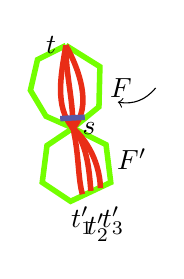
\begin{tikzpicture}[scale=.6]
\draw[green!55!yellow,line width=2pt](0,2)--(-.6,1.7)--(-.75,1.05)--(-.42,.5)--(.15,.25)--(.7,.7)--(.72,1.55)--(0,2);
\draw[green!55!yellow,line width=2pt](.15,.25)--(-.4,-.12)--(-.5,-.9)--(.1,-1.3)--(.95,-.9)--(.85,-.1)--(.15,.25);
\draw[red!65!brown,line width=2pt](0,2)..controls(-.1,1.4)and(-.25,.7)..(.15,.25)..controls(.28,-.3)and(.25,-.8)..(.35,-1.15);
\draw[red!65!brown,line width=2pt](0,2)..controls(.28,1.5)and(.57,.7)..(.15,.25)..controls(.65,-.2)and(.73,-.8)..(.73,-1.02);
\draw[red!65!brown,line width=2pt](0,2)..controls(.0,1.35)and(.15,.9)..(.15,.25)..controls(.48,-.1)and(.5,-.8)..(.53,-1.08);
\draw[blue!30!gray,line width=2pt](-.12,.45)--(.4,.48);
\node[left]at(0,2){\(t\)};\node[right]at(.15,.25){\(s\)};
\node[right]at(.73,1.1){\(F\)};\node[right]at(.88,-.4){\(F'\)};
\node[below]at(.35,-1.2){\(t'_1\)};\node[below]at(.68,-1.35){\(t'_2\)};\node[below]at(1,-1.2){\(t'_3\)};
\draw[->](1.9,1.1)to[bend left](1.1,.8);
\end{tikzpicture}}

% E: text|bottom right, k|Appelons un côté exceptionnel
k) Appelons un côté exceptionnel \uline{stable} ou instable (ou semi-stable) suivant que les deux \deleted{positions relatives} \inserted{\unsure{faces}} incidences correspondent à des p.r. stables (resp. instables) (condition \unsure{toujours} \unsure{top.}\unsure{ment} \unsure{forcée}). Nous \unsure{prendrons} le \unsure{sommet} exceptionnel le bord privilégié de la branche ord. de \(K\) qui y passe et des côtés en \unsure{bouts} exc. instables (\unsure{non forcé}).
\mspage{45}
